\subsection{Caso d'uso UC3: Gestione della presentazione}
\begin{figure}[h] 
	\centering 
	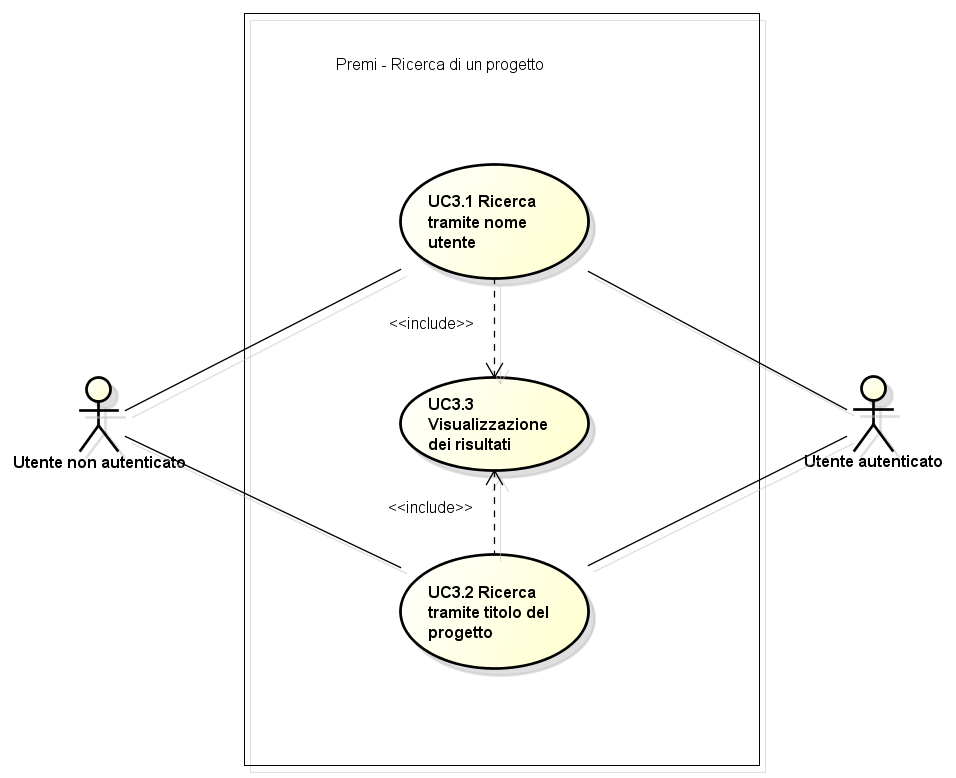
\includegraphics[scale=0.45] {img/UC3.png} 
	\caption{UC3 - Gestione della presentazione} 
\end{figure}

\begin{itemize}
	\item \textbf{Attori:} Utente;
	\item \textbf{Scopo e descrizione:} L'utente sta lavorando su una presentazione per creare delle nuove slide o per modificare quelle già create. Può quindi inserire le seguente cose: slide, immagini, caselle di testo, dati real time, tabelle. Ha inoltre la possibilità di modificare gli elementi inseriti, oppure di eliminarli. Può infine scegliere l'effetto di transizione da una slide ad un'altra;
	\item \textbf{Precondizione:} Il sistema mostra la schermata di gestione di una presentazione e l'utente vuole creare/modificare una slide;
	\item \textbf{Flusso degli eventi:}
	\begin{enumerate}
		\item L'utente può inserire una nuova slide [UC3.1];
		
		\item L'utente può inserire un'immagine [UC3.2];
		\item L'utente carica un file per inserire l'immagine [UC3.12];
		
		\item L'utente può inserire una casella di testo [UC3.3];
		\item L'utente sceglie la formattazione del testo [UC3.13];
		
		\item L'utente può inserire dati real time [UC3.4];
		
		\item L'utente può inserire una tabella [UC3.5];
		\item L'utente può modificare una tabella [UC3.13];
		
		\item L'utente può inserire un grafico [UC3.6];
		\item L'utente può personalizzare un grafico [UC3.15];
		
		\item L'utente può scegliere un effetto di transizione [UC3.7];
		
		\item L'utente può cambiare dimensione all'elemento [UC3.8];
		
		\item L'utente può cambiare posizione all'elemento [UC3.9];
		
		\item L'utente può ruotare l'elemento [UC3.10];
		
		\item L'utente può rimuovere l'elemento [UC3.11].
	\end{enumerate}
	\item \textbf{Postcondizione:} Il sistema mostra le operazioni effettuate dall'utente.
\end{itemize}

\subsection{Caso d'uso UC3.1: Inserire una nuova slide}
\begin{itemize}
	\item \textbf{Attori:} Utente;
	\item \textbf{Scopo e descrizione:} L'utente crea una nuova slide nella presentazione per poter inserire del contenuto;
	\item \textbf{Precondizione:} Il sistema è in attesa che l'utente crei una nuova slide;
	\item \textbf{Postcondizione:} Il sistema ha creato la nuova slide.
\end{itemize}

\subsection{Caso d'uso UC3.2: Inserire un'immagine}
\begin{itemize}
\item \textbf{Attori:} Utente;
\item \textbf{Scopo e descrizione:} L'utente deve inserire l'immagine da mettere nella slide;
\item \textbf{Precondizione:} Il sistema è in attesa che l'utente selezioni l'immagine;
\item \textbf{Postcondizione:} Il sistema ha caricato l'immagine selezionata dall'utente.
\end{itemize}

\subsection{Caso d'uso UC3.3: Inserire una casella di testo}
\begin{itemize}
\item \textbf{Attori:} Utente;
\item \textbf{Scopo e descrizione:} L'utente deve inserire una casella di testo nella slide;
\item \textbf{Precondizione:} Il sistema è in attesa che l'utente crei una casella di testo;
\item \textbf{Postcondizione:} Il sistema ha creato la casella di testo.
\end{itemize}

\subsection{Caso d'uso UC3.4: Inserire dati real time}
\begin{itemize}
	\item \textbf{Attori:} Utente;
	\item \textbf{Scopo e descrizione:} L'utente deve inserire dei dati real time;
	\item \textbf{Precondizione:} Il sistema è in attesa che l'utente inserisca i dati real time;
	\item \textbf{Postcondizione:} Il sistema ha inserito i dati real time.
\end{itemize}

\subsection{Caso d'uso UC3.5: Inserire una tabella}
\begin{itemize}
	\item \textbf{Attori:} Utente;
	\item \textbf{Scopo e descrizione:} L'utente deve inserire una tabella;
	\item \textbf{Precondizione:} Il sistema è in attesa che l'utente inserisca una tabella;
	\item \textbf{Postcondizione:} Il sistema ha inserito la tabella.
\end{itemize}


\subsection{Caso d'uso UC3.6: Inserire un grafico}
\begin{itemize}
	\item \textbf{Attori:} Utente;
	\item \textbf{Scopo e descrizione:} L'utente deve inserire un grafico;
	\item \textbf{Precondizione:} Il sistema è in attesa che l'utente inserisca un grafico;
	\item \textbf{Postcondizione:} Il sistema ha inserito il grafico.
\end{itemize}

\subsection{Caso d'uso UC3.7: Scegliere un effetto di transizione}
\begin{itemize}
	\item \textbf{Attori:} Utente;
	\item \textbf{Scopo e descrizione:} L'utente deve scegliere l'effetto di transizione da dare alla slide;
	\item \textbf{Precondizione:} Il sistema è in attesa che l'utente selezioni l'effetto desiderato;
	\item \textbf{Postcondizione:} Il sistema ha inserito l'effetto di transizione.
\end{itemize}

\subsection{Caso d'uso UC3.8: Ridimensionamento di un elemento}
\begin{itemize}
	\item \textbf{Attori:} Utente;
	\item \textbf{Scopo e descrizione:} L'utente cambia la grandezza dell'elemento selezionato della slide;
	\item \textbf{Precondizione:} Il sistema mostra l'elemento selezionato che si intende ridimensionare;
	\item \textbf{Postcondizione:} Il sistema ha ridimensionato l'elemento della slide.
\end{itemize}

\subsection{Caso d'uso UC3.9: Spostamento di un elemento}
\begin{itemize}
	\item \textbf{Attori:} Utente;
	\item \textbf{Scopo e descrizione:} L'utente cambia la posizione dell'elemento selezionato della slide;
	\item \textbf{Precondizione:} Il sistema mostra l'elemento selezionato che si intende spostare;
	\item \textbf{Postcondizione:} Il sistema ha spostato l'elemento della slide.
\end{itemize}

\subsection{Caso d'uso UC3.10: Rotazione di un elemento}
\begin{itemize}
	\item \textbf{Attori:} Utente;
	\item \textbf{Scopo e descrizione:} L'utente ruota l'elemento selezionato della slide;
	\item \textbf{Precondizione:} Il sistema mostra l'elemento selezionato che si intende ruotare;
	\item \textbf{Postcondizione:} Il sistema ha ruotato l'elemento della slide.
\end{itemize}

\subsection{Caso d'uso UC3.11: Rimozione di un elemento}
\begin{itemize}
	\item \textbf{Attori:} Utente;
	\item \textbf{Scopo e descrizione:} L'utente elimina l'elemento selezionato dalla slide;
	\item \textbf{Precondizione:} Il sistema mostra l'elemento selezionato che si intende cancellare;
	\item \textbf{Postcondizione:} Il sistema ha cancellato l'elemento dalla slide.
\end{itemize}

\subsection{Caso d'uso UC3.12: Caricare un file}
\begin{itemize}
	\item \textbf{Attori:} Utente;
	\item \textbf{Scopo e descrizione:} L'utente deve caricare un file da utilizzare nella presentazione;
	\item \textbf{Precondizione:} Il sistema è in attesa che l'utente selezioni il file;
	\item \textbf{Postcondizione:} Il sistema ha caricato il file selezionato dall'utente e lo ha inserito nella slide.
\end{itemize}

\subsection{Caso d'uso UC3.13: Scegliere la formattazione del testo}
\begin{figure}[h] 
	\centering 
	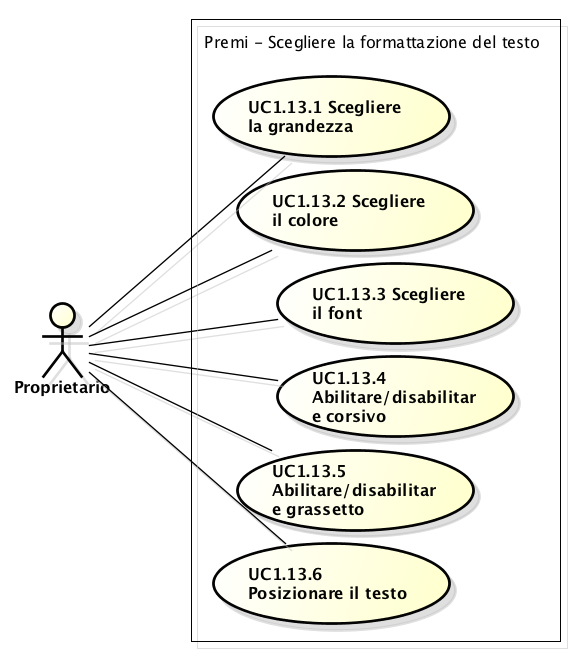
\includegraphics[scale=0.45] {img/UC3.13.png} 
	\caption{UC3.13 - Scegliere la formattazione del testo}
\end{figure}

\begin{itemize}
	\item \textbf{Attori:} Utente;
	\item \textbf{Scopo e descrizione:} L'utente può modificare l'aspetto del testo contenuto in una casella di testo. L'utente seleziona il testo e poi sceglie che modifiche effettuare;
	\item \textbf{Precondizione:} Il sistema è in attesa che l'utente selezioni la modifica da apportare al testo e il testo da modificare è selezionato;
	\item \textbf{Flusso degli eventi:}
	\begin{enumerate}
		\item L'utente può cambiare la grandezza del testo [UC3.13.1];
		\item L'utente può cambiare il colore del testo [UC3.13.2];
		\item L'utente può cambiare il font del testo [UC3.13.3];
		\item L'utente può abilitare o disabilitare il testo in corsivo [UC3.13.4];
		\item L'utente può abilitare o disabilitare il testo in grassetto [UC3.13.5];
		\item L'utente può spostare il testo in una nuova posizione [UC3.13.6].
	\end{enumerate}
	\item \textbf{Postcondizione:} Il sistema ha apportato le modifiche scelte al testo.
\end{itemize}

\subsection{Caso d'uso UC3.13.1: Scegliere la grandezza}
\begin{itemize}
	\item \textbf{Attori:} Utente;
	\item \textbf{Scopo e descrizione:} L'utente può cambiare la grandezza del testo;
	\item \textbf{Precondizione:} Il testo da modificare è selezionato;
	\item \textbf{Postcondizione:} Il testo è stato ingrandito o rimpicciolito secondo la scelta dell'utente.
\end{itemize}

\subsection{Caso d'uso UC3.13.2: Scegliere il colore}
\begin{itemize}
	\item \textbf{Attori:} Utente;
	\item \textbf{Scopo e descrizione:} L'utente può cambiare il colore del testo;
	\item \textbf{Precondizione:} Il testo da modificare è selezionato;
	\item \textbf{Postcondizione:} Il testo è stato colorato secondo la scelta dell'utente.
\end{itemize}

\subsection{Caso d'uso UC3.13.3: Scegliere il font}
\begin{itemize}
	\item \textbf{Attori:} Utente;
	\item \textbf{Scopo e descrizione:} L'utente può cambiare il font del testo;
	\item \textbf{Precondizione:} Il testo da modificare è selezionato;
	\item \textbf{Postcondizione:} Il testo ha cambiato font secondo la scelta dell'utente.
\end{itemize}

\subsection{Caso d'uso UC3.13.4: Abilitare/disabilitare corsivo}
\begin{itemize}
	\item \textbf{Attori:} Utente;
	\item \textbf{Scopo e descrizione:} L'utente può abilitare o disabilitare la scrittura in corsivo;
	\item \textbf{Precondizione:} Il testo da modificare è selezionato oppure è stata selezionata la casella di testo nella quale poter scrivere;
	\item \textbf{Postcondizione:} Il testo è stato modificato secondo la scelta dell'utente.
\end{itemize}

\subsection{Caso d'uso UC3.13.5: Abilitare/Disabilitare grassetto}
\begin{itemize}
	\item \textbf{Attori:} Utente;
	\item \textbf{Scopo e descrizione:} L'utente può abilitare o disabilitare la scrittura in grassetto;
	\item \textbf{Precondizione:} Il testo da modificare è selezionato oppure è stata selezionata la casella di testo nella quale poter scrivere;
	\item \textbf{Postcondizione:} Il testo è stato modificato secondo la scelta dell'utente.
\end{itemize}

\subsection{Caso d'uso UC3.13.6: Posizionare il testo}
\begin{itemize}
	\item \textbf{Attori:} Utente;
	\item \textbf{Scopo e descrizione:} L'utente può spostare una casella di testo in una nuova posizione;
	\item \textbf{Precondizione:} La casella di testo da spostare è stata selezionata;
	\item \textbf{Postcondizione:} La casella di testo è stata spostata secondo la scelta dell'utente.
\end{itemize}

\subsection{Caso d'uso UC3.14: Modificare una tabella}
\begin{figure}[h] 
	\centering 
	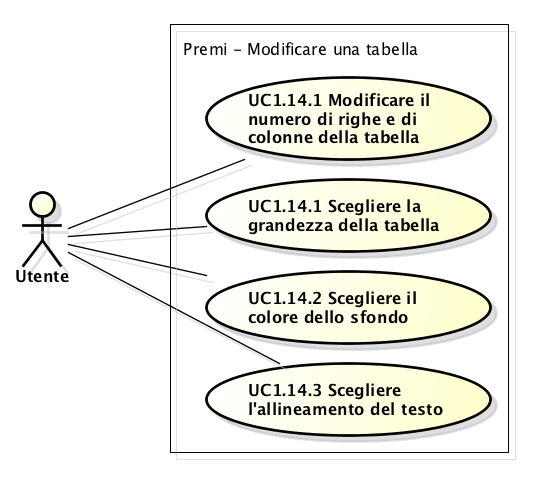
\includegraphics[scale=0.45] {img/UC3.14.png} 
	\caption{UC3.14 - Modificare una tabella} 
\end{figure}

\begin{itemize}
	\item \textbf{Attori:} Utente;
	\item \textbf{Scopo e descrizione:} L'utente può modificare l'aspetto della tabella e del suo contenuto. L'utente seleziona la tabella o il testo e poi sceglie che modifiche effettuare;
	\item \textbf{Precondizione:} Il sistema è in attesa che l'utente selezioni la modifica da apportare alla tabella e la tabella o il testo da modificare sono selezionati;
	\item \textbf{Flusso degli eventi:}
	\begin{enumerate}
		\item L'utente può modificare il numero di righe e di colonne [UC3.14.1]
		\item L'utente può cambiare la grandezza della tabella [UC3.14.2];
		\item L'utente può cambiare il colore di sfondo della tabella [UC3.14.3];
		\item L'utente può cambiare l'allineamento del testo [UC3.14.4];
		\item L'utente può cambiare la formattazione del testo [UC3.13];
	\end{enumerate}
	\item \textbf{Postcondizione:} Il sistema ha apportato le modifiche scelte alla tabella.
\end{itemize}

\subsection{Caso d'uso UC3.14.1: Modificare il numero di righe e colonne della tabella}
\begin{itemize}
	\item \textbf{Attori:} Utente;
	\item \textbf{Scopo e descrizione:} L'utente può modificare la grandezza della tabella;
	\item \textbf{Precondizione:} La tabella da modificare è stata selezionata;
	\item \textbf{Postcondizione:} La tabella è stata modificata nelle sue dimensioni secondo la scelta dell'utente.
\end{itemize}

\subsection{Caso d'uso UC3.14.2: Scegliere grandezza della tabella}
\begin{itemize}
	\item \textbf{Attori:} Utente;
	\item \textbf{Scopo e descrizione:} L'utente può modificare la grandezza della tabella;
	\item \textbf{Precondizione:} La tabella da modificare è stata selezionata;
	\item \textbf{Postcondizione:} La tabella è stata modificata nelle sue dimensioni secondo la scelta dell'utente.
\end{itemize}

\subsection{Caso d'uso UC3.14.3: Scegliere colore di sfondo della tabella}
\begin{itemize}
	\item \textbf{Attori:} Utente;
	\item \textbf{Scopo e descrizione:} L'utente può modificare il colore di sfondo della tabella;
	\item \textbf{Precondizione:} La tabella o le celle da modificare sono state selezionate;
	\item \textbf{Postcondizione:} Lo sfondo della tabella o delle celle è stato modificato secondo la scelta dell'utente.
\end{itemize}

\subsection{Caso d'uso UC3.14.4: Scegliere allineamento del testo}
\begin{itemize}
	\item \textbf{Attori:} Utente;
	\item \textbf{Scopo e descrizione:} L'utente può modificare l'allineamento del testo della tabella;
	\item \textbf{Precondizione:} La tabella o le celle da modificare sono state selezionate;
	\item \textbf{Postcondizione:} L'allineamento del testo della tabella o delle celle è stato modificato secondo la scelta dell'utente.
\end{itemize}

\subsection{Caso d'uso UC3.15: Personalizzare un grafico}
\begin{figure}[h] 
	\centering 
	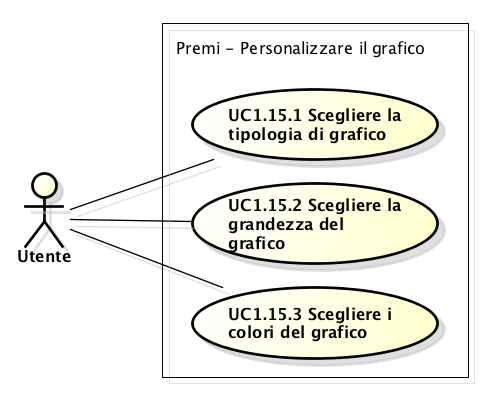
\includegraphics[scale=0.45] {img/UC3.15.png} 
	\caption{UC3.15 - Personalizzare un grafico} 
\end{figure}

\begin{itemize}
	\item \textbf{Attori:} Utente;
	\item \textbf{Scopo e descrizione:} L'utente può modificare la tipologia e l'aspetto del grafico o del suo contenuto. L'utente seleziona il grafico e poi sceglie che modifiche effettuare;
	\item \textbf{Precondizione:} Il sistema è in attesa che l'utente selezioni la modifica da apportare al grafico e il grafico da modificare è selezionato;
	\item \textbf{Flusso degli eventi:}
	\begin{enumerate}
		\item L'utente può cambiare la tipologia del grafico [UC3.15.1];
		\item L'utente può cambiare la dimensione del grafico [UC3.15.2]
		\item L'utente può cambiare i colori del grafico [UC3.15.3];
	\end{enumerate}
	\item \textbf{Postcondizione:} Il sistema ha apportato le modifiche scelte al grafico.
\end{itemize}

\subsection{Caso d'uso UC3.15.1: Scegliere la tipologia del grafico}
\begin{itemize}
	\item \textbf{Attori:} Utente;
	\item \textbf{Scopo e descrizione:} L'utente può modificare la tipologia del grafico;
	\item \textbf{Precondizione:} Il grafico da modificare è stata selezionato;
	\item \textbf{Postcondizione:} La tipologia del grafico è stata modificata secondo la scelta dell'utente.
\end{itemize}

\subsection{Caso d'uso UC3.15.2: Scegliere la grandezza del grafico}
\begin{itemize}
	\item \textbf{Attori:} Utente;
	\item \textbf{Scopo e descrizione:} L'utente può modificare la grandezza del grafico;
	\item \textbf{Precondizione:} Il grafico da modificare è stata selezionato;
	\item \textbf{Postcondizione:} Il grafico è stata modificato nelle sue dimensioni secondo la scelta dell'utente.
\end{itemize}

\subsection{Caso d'uso UC3.15.3: Scegliere i colori del grafico}
\begin{itemize}
	\item \textbf{Attori:} Utente;
	\item \textbf{Scopo e descrizione:} L'utente può modificare il set di colori del grafico;
	\item \textbf{Precondizione:} Il grafico da modificare è stata selezionato;
	\item \textbf{Postcondizione:} I colori del grafico sono stati modificati secondo la scelta dell'utente.
\end{itemize}